\section{Versuchsaufbau/-durchführung}
Nachfolgend soll nun genauer die Funktionsweise eines Germaniumdetektors erklärt werden. 
Hierbei wird weniger auf elektrotechnische Details 
als auf die messtechnische Motivation der einzelnen Bauteile eingegangen.
Anschließend werden die durchgeführten Messungen vorgestellt.

Der Germanium-Detektor verfügt über eine zylindrische Geometrie, die in Abbildung~\ref{fig: geometrie} dargestellt ist. 
Von Außen ist eine stark mit Lithium dotierte $n$
Schicht aufgebracht, von Innen eine mit Gold dotierte $p$ Schicht. An die Schichten sind Elektroden angeschlossen, zwischen denen 
die notwendige Hochspannung von $\SI{5}{\kilo\volt}$ angelegt ist. Die Probe wird über dem Zylinder in eine Schraubvorrichtung 
befestigt. Probe und Detektor befinden sich innerhalb einer sogenannten Bleiburg, die z.\,B. den Einfluss von kosmischer 
Strahlung minimieren soll. Zudem schützt eine innere dünne Kupferschicht vor Strahlung, die von der Bleiummantelung ausgehen 
könnte. 
\begin{figure}
\centering
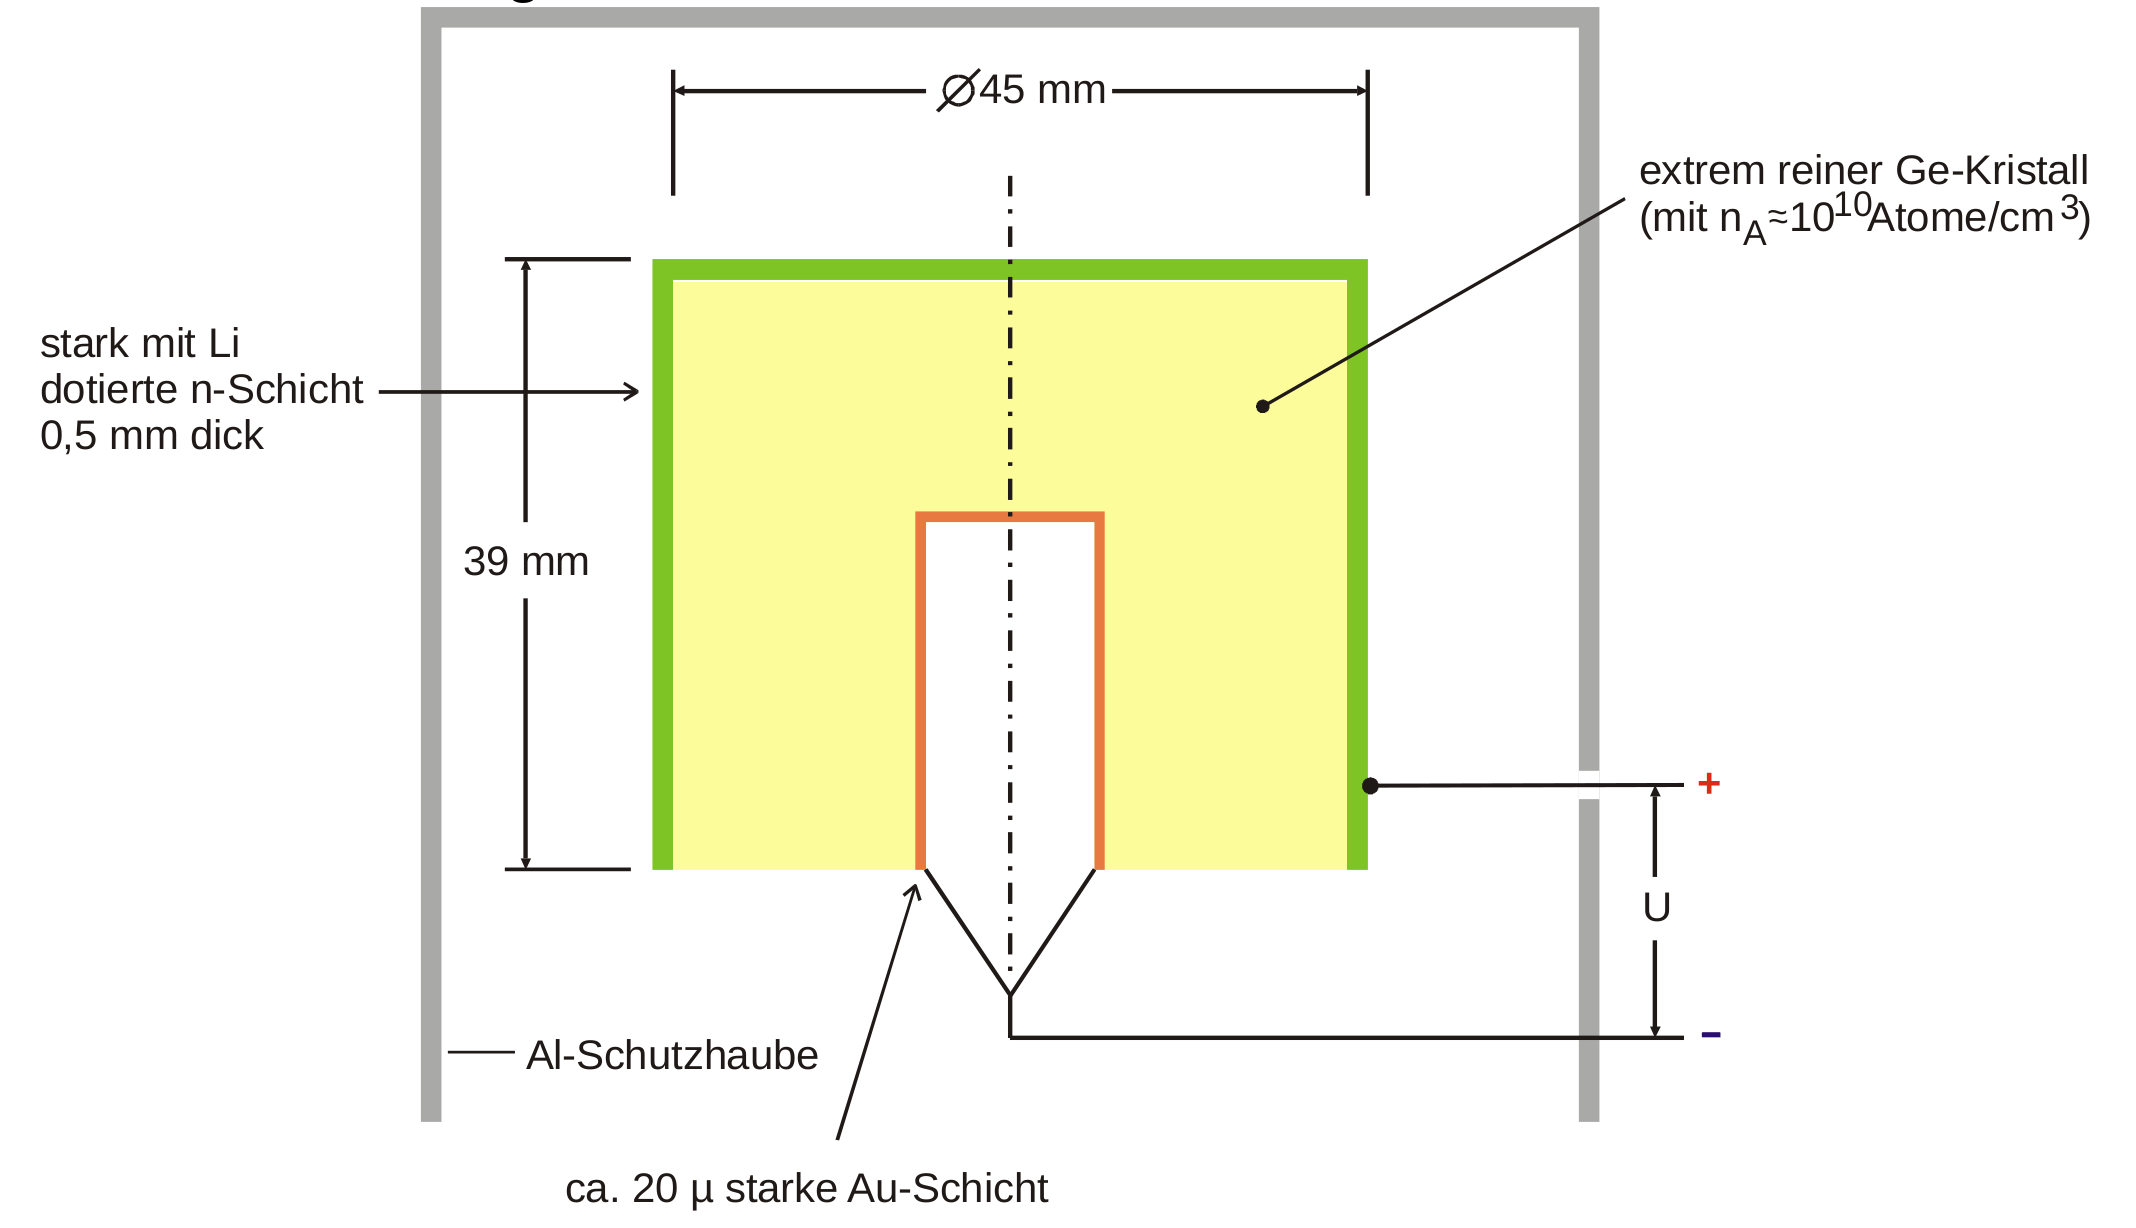
\includegraphics[width = 0.8\textwidth]{pics/geometrie.png}
\caption{Querschnitt durch den Koaxialen Germanium-Detektor zur Veranschaulichung der verwendeten Geometrie~\cite{anleitungv18}.}
\label{fig: geometrie}
\end{figure}

Der am Halbleiterelement erzeugte Stromimpuls muss zunächst in einen Spannungsimpuls umgewandelt werden. Dies geschieht mit 
dem Vorverstärker in Abbildung~\ref{fig: vorverstaerker}(a). Mithilfe eines kapazitiv rückgekoppelten Operationsverstärkers wird durch elektrische 
Integration ein Spannungspegel erzeugt, der proportional zur Photonenenergie seien soll. Um einen zeitlich 
begrenzten Spannungsimpuls zu erhalten, ist der Kondensator $C_K$ nach jedem Nachweis zu entladen, was durch die 
Anordnung in Abbildung~\ref{fig: vorverstaerker}(b) erfolgt. Durch eine LED wird nach jedem Impuls die Gate-Drain-Schicht des 
Eingangs-Feldeffekttransistors (FET) leitend gemacht und so kann die Ladung von $C_K$ abfließen.
\begin{figure}
\centering
\begin{subfigure}{0.49\textwidth}
\centering
\includegraphics[width = \textwidth]{pics/vorverstärker.pdf}
\end{subfigure}
\begin{subfigure}{0.49\textwidth}
\centering
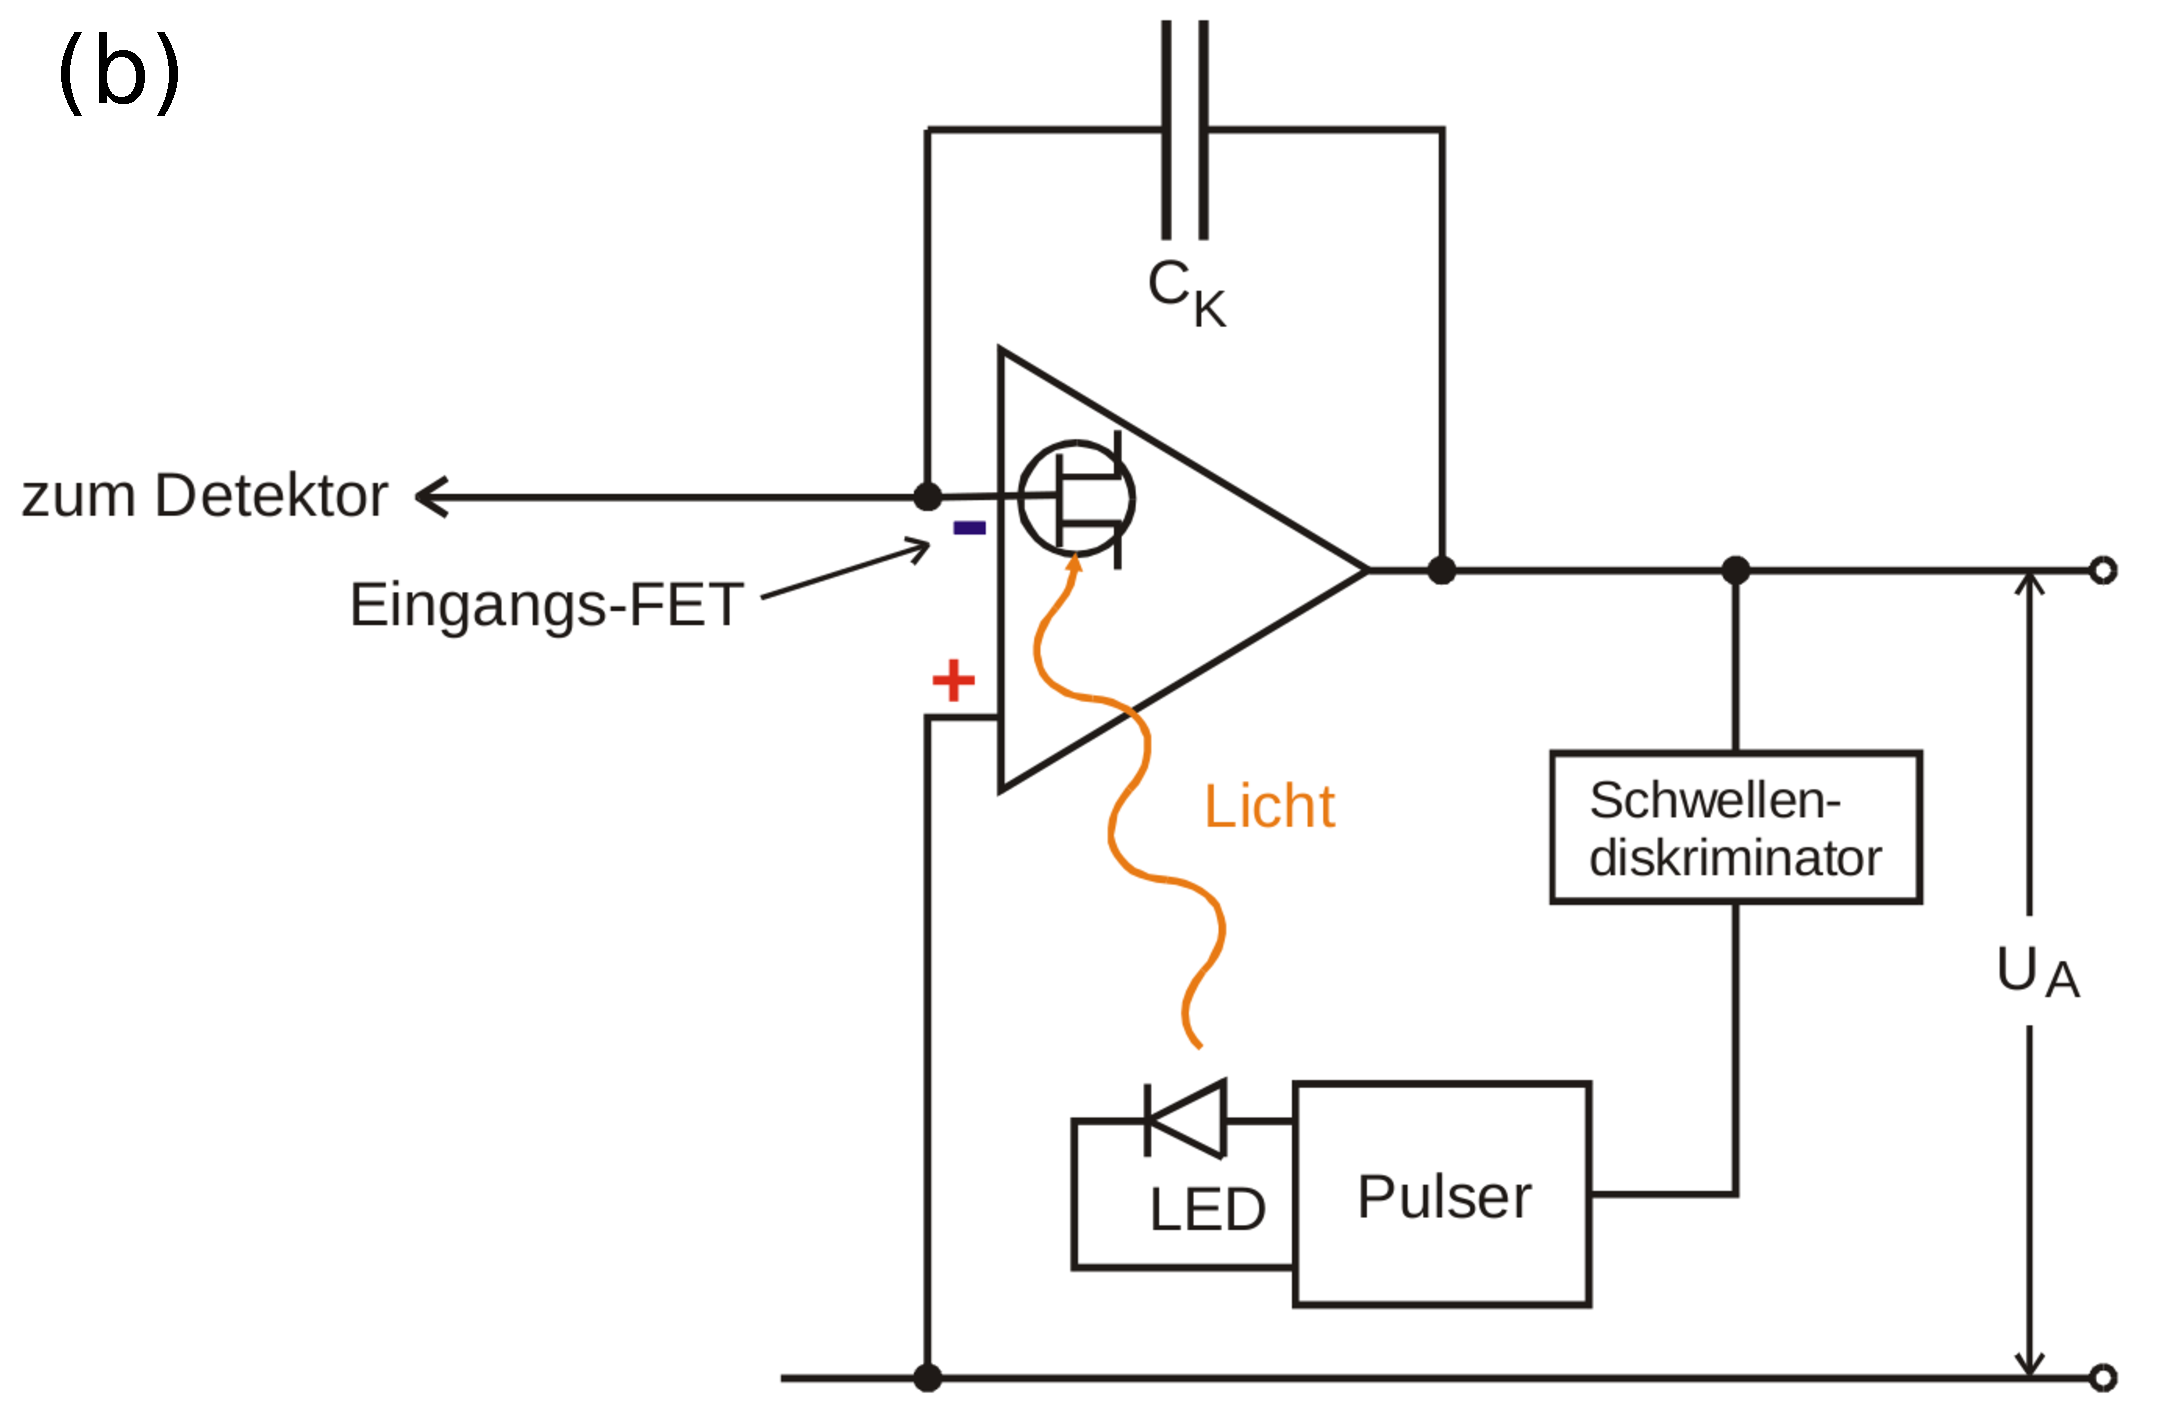
\includegraphics[width = \textwidth]{pics/led.pdf}
\end{subfigure}
\caption{(a) Schlatplan des Vorverstärkers. (b) Schaltung zum Entladen des integrierenden Kondensators mittels einer LED.
Beide Abbildungen (bearbeitet) aus \cite{anleitungv18}.}
\label{fig: vorverstaerker}
\end{figure}

Das vorverstärkte Signal gelangt zu einem Hauptverstärker, der die Spannungsimpulse abschließend verstärkt, sodass 
sie vom Vielkanalanalysator in Kanäle eingeordnet werden können. Vor- und Hauptverstärker sind über ein RC-Glied (dient hier als Hochpass)
miteinander gekoppelt, um Offsetspannungen nicht ebenfalls zu verstärken. Da die Zeitkonstante $RC$ im Allgemeinen ungleich 
$C_K R_K$ (siehe Abbildung\ref{}) ist, kann es hierdurch jedoch zu Unterschwingungen $U < 0$ des Signals kommmen. Ein gleicher Effekt kann 
am Ausgang des Hauptverstärkers entstehen. Der Detektor wird in dieser Zeit unempfindlicher auf ein neues Signal. Der Aufbau enthält 
elektrotechnische Lösungen (Pole-Zero-Kompensation und Base-Line-Restorer), die hier nur benannte werden sollen. Ein weiteres Problem tritt auf, wenn 
zu viele Impulse in zu kurzer Zeit eingehen, die dann als einzelner Verstärkter Impuls regestriert werden (Pile-Up). Auch solche Signale 
können erkannt und blockiert werden, was jedoch zu einer Totzeit, bzw. einer Verminderung der Gesamtzählrate führt.


Die eigentliche Zählung der Spannungsimpulse geschieht über eine Schaltung, wie sie in 
Abbildung~\ref{fig: zaehler}
dargestellt ist. Die Messung der Impulshöhe basiert hier auf einer Zeitmessung. Der Spannungsimpuls lädt einen 
Kondensator auf, dessen Abklingszeit bei Entladung von der Amplitude des Pulses abhängt. Ein Und-Gatter, verknüpft 
das zu untersuchende Signal mit einem Quarzoszillator. Die Zählrate am Binärzähler ist damit ein direktes Maß für 
die Impulshöhe und somit auch für die Energie der Photonen. 
Die Zählraten werden abschließend in einem Computer verarbeitet und als Ergebnis wird ein Histogramm erzeugt, auf dessen 
$x$-Achse Kanalnummern sind und auf der $y$-Achse die Anzahl der Ereignisse $Z$ für jeden Kanal. 
Ein letzte wichtige Größe zur Charakterisierung des Detektors ist 
die Effizienz $Q$. Mit dieser, der Emissionswahrscheinlichkeit $W$, der Aktivität $A$ des Strahlers lässt sich die 
Zählrate $Z$ berechnen 
\begin{equation}
    Z = \frac{\Omega}{4\pi} A \, W \, Q.
    \label{eq: zählrate}
\end{equation}
Der Raumwinkelanteil $\frac{\Omega}{4\pi}$, in dem Strahlung der Quelle in den Detektor gelangt, lässt sich annähernd (Abstand zwischen 
Detektor und Probe groß im Vergleich zur Abmessung der Probe) bestimmen zu 
\begin{equation}
    \frac{\Omega}{4\pi} = \frac{1}{2} \left( 1 - \frac{a}{\sqrt{a^2 + r^2}} \right),
    \label{eq: omega}
\end{equation}
mit dem Radius des oben beschriebenen Zylinders $r$ und dem Abstand $a$ zwischen Probe und Zylinderdeckelfläche. 
\begin{figure}
    \centering
    \includegraphics[width = 0.8\textwidth]{pics/zähler.pdf}
    \caption{Schaltung zur Einordnung der Spannungspulse in Abhängigkeit ihrer Amplitude. Abbildung aus \cite{anleitungv18}.}
    \label{fig: zaehler}
\end{figure}

Für alle Messungen wird für etwa eine Stunde eine Probe in den Detektor gebracht und ein Spektrum aufgenommen. In der 
Auswertung kann dann auf die Messzeit normiert werden. 
Zunächst muss herausgefunden werden, welcher Zusammenhang zwischen Kanalnummer und Energie, sowie zwischen Zählrate und 
Intensität besteht. Hierzu wird zunächst eine \ce{^152Eu} Quelle untersucht. Diese besitzt ein Linien-reiches Spektrum, für das 
die Energien und notwendige Größen in Formel~\eqref{eq: zählrate} bekannt sind. 
Anschließend wird eine \ce{^137Cs} untersucht. Hiermit sollen insbesondere die Eigenschaften aus 
Abbildung~\ref{fig: example_spectrum} quantitativ untersucht werden. Hierzu zählen z.B. Lage von Compton-Kante und 
Rückstreupeak. Ebenfalls relevant ist das energetische Auflösungsvermögen des Systems, das aus einer Untersuchung der Breite 
des Gesamtenergiepeaks hervorgeht. Das Auflösungsvermögen bestimmt die Unterscheidbarkeit zweier Linien im Spektrum und kann durch 
die Halbwertbreite $\Delta E_{\sfrac{1}{2}}$ eines Peaks quantifiziert werden. Hierfür lässt sich zeigen, dass diese 
näherungsweise bestimmt ist durch die Photonenenergie $E_\gamma$ und die Anregungsenergie $E_{el}$ eines Elektrons im Germanium 
\begin{equation}
    \Delta E_{\sfrac{1}{2}} = \num{2.35}\sqrt{\num{0.1}E_\gamma E_{el}}
    \label{eq: E_fwhm}
\end{equation}

Abschließend werden zwei Messungen durchgeführt die von der generischen Situation der Gamma-Spektrometrie ausgehen: 
Die Quelle ist nicht bekannt und anhand des Spektrums soll heraus gefunden werden, worum es sich handelt. Bei der ersten 
Probe handelt es sich entweder um \ce{^125 Sb} oder \ce{^133Ba}, die letzte Quelle ist gänzlich unbekannt.